\chapter{Lipkin-Meshkov Glick model}
The Lipkin-Meshkov Glick model is a simple model manifesting the quantum phase transitions. The aim of this chapter is to understand the properties of the ground state and see its influence on different driving protocols.


The model is defined by Hamiltonian
\begin{equation}
    \HH=\J_3+\lambda\hat V_1 +\chi \hat V_2+\chi^2 \hat V_3,
    \label{eq:firstOrderTransitionHamiltonian}
\end{equation}
where
\begin{align}
    \hat V_1 &=-\frac{1}{2j}\J_1^2\\
    \hat V_2 &= -\frac{1}{2j}\left[\J_1(\J_3+j\Id)+(\J_3+j\Id)\J_1\right]\\
    \hat V_3 &= -\frac{1}{2j}(\J_3+j\Id)^2.
\end{align}



Using the Spherical harmonics basis $\{\ket{j,m}\}$ for quantum numbers $j$ as the angular momentum and $m$ its projection on the direction of $\J_3$ and defining
\begin{equation}
    \J_\pm\coloneqq\frac{1}{2}(\J_1\pm i\J_2),
\end{equation}
we get the matrix elements
\begin{align}
    \braket{j'm'|\J^2|jm} &= j(j+1)\delta_{j'j}\delta_{m'm}\\
    \braket{j'm'|\J_3|jm} &= m \delta_{j'j}\delta_{m'm}\\
    \braket{j'm'|\J_\pm|jm} &= \sqrt{(j\mp m)(j\pm m+1)}\delta_{j'j}\delta_{m'm\pm 1},
\end{align}
where $\delta_{a'b}$ is Kronecker delta. The Hamiltonian in Eq. \ref{eq:firstOrderTransitionHamiltonian} can be written as
\begin{equation}
\begin{split}
        % \left(\J_1+\chi(\J_3+j)\right)^2 &= \textcolor{purple}{\J_1^2} +\chi^2 (\J_3^2+j^2\Id+2j\J_3)+\chi(\textcolor{blue}{\J_1}\J_3+\J_3\textcolor{blue}{\J_1})+2\chi j\textcolor{blue}{\J_1}\\
        % \textcolor{purple}{\J_1^2}&= \frac{1}{4}(\J_++\J_-)^2= \frac{1}{4}(\J_+^2+\J_-^2+\textcolor{violet}{\J_+\J_-}+\textcolor{violet}{\J_-\J_+})\\ 
        % \textcolor{violet}{\J_\pm\J_\mp}&=\J^2-\J_3^2 \mp \J_3\\
        % \textcolor{blue}{\J_1}&=(\J_+ +\J_-),\\
        \HH =& J_3-\frac{\lambda}{8j}(J_++J_-)^2-\frac{\chi}{4j}\left[(J_++J_-)(J_3+j\Id)+(J_3+j\Id)(J_++J_-)\right]\\
        &-\frac{\chi^2}{2j}(J_3+j\Id)^2,
\end{split}
\end{equation}
which has pentadiagonal matrix representation. During the whole paper, $j=N/2$ will be used. 











\section{Special cases}
Because of pentadiagonal character of the Hamiltonian, the discussion will start at $N=3$, followed by $N=5$. Then the limit $N\rightarrow\infty$ will be taken along with the generalization of some characteristics to an arbitrary dimension. 

Due to the complexity of our Hamiltonian, it is not possible to prove every statement analytically. Some numerical methods, supported by some basic theorems, are needed.



\subsection{Case $N=3$}
The lowest dimension behaving similarly to higher $N$ is 3 with the matrix represented Hamiltonian
\begin{equation}
    \HH=\left(
        \begin{array}{cccc}
         -\frac{ \lambda +6}{4} & -\frac{\chi }{2 \sqrt{3}} & -\frac{\lambda }{2 \sqrt{3}} & 0 \\
         -\frac{\chi }{2 \sqrt{3}} & \frac{ \left(-7 \lambda -4 \chi ^2-6\right)}{12} & -\chi  & -\frac{\lambda }{2 \sqrt{3}} \\
         -\frac{\lambda }{2 \sqrt{3}} & -\chi  & \frac{ \left(-7 \lambda -16 \chi ^2+6\right)}{12} & -\frac{5 \chi }{2 \sqrt{3}} \\
         0 & -\frac{\lambda }{2 \sqrt{3}} & -\frac{5 \chi }{2 \sqrt{3}} & -\frac{\lambda }{4}-3 \chi ^2+\frac{3}{2} \\
        \end{array}
        \right).
\end{equation}
The spectrum of this Hamiltonian can be calculated analytically using some complex functions $D, E, F, G:\C\rightarrow \C$, see Appendix \ref{appendix1}, as
\begin{align}
        E_0 &= \frac{1}{12} \left(G-F-\frac{\sqrt{D-E}}{2}\right)
        \label{eq:N=3_en0}\\
        E_1 &= \frac{1}{12}  \left(G-F+\frac{\sqrt{D-E}}{2}\right)
        \label{eq:N=3_en1}\\
        E_2 &= \frac{1}{12} \left(G+F-\frac{\sqrt{D+E}}{2}\right)
        \label{eq:N=3_en2}\\
        E_3 &= \frac{1}{12}  \left(G+F+\frac{\sqrt{D+E}}{2}\right).
        \label{eq:N=3_en3}
\end{align}
Eigenvectors can also be written analytically, but doing it here would be redundant. On sections $\lambda=1$ and $\chi=1$, see Figures \ref{fig:N=3_energiesl} resp. \ref{fig:N=3_energiesc}, it can be seen the general behavior of the spectrum, where the energies get close to each other somewhere around the center of our coordinate system $(\lambda;\chi)$ and then separate monotonously to never meet again. In addition, the spectrum is symmetrical for $\chi\leftrightarrow -\chi$.
\begin{figure}[H]
    \centering
    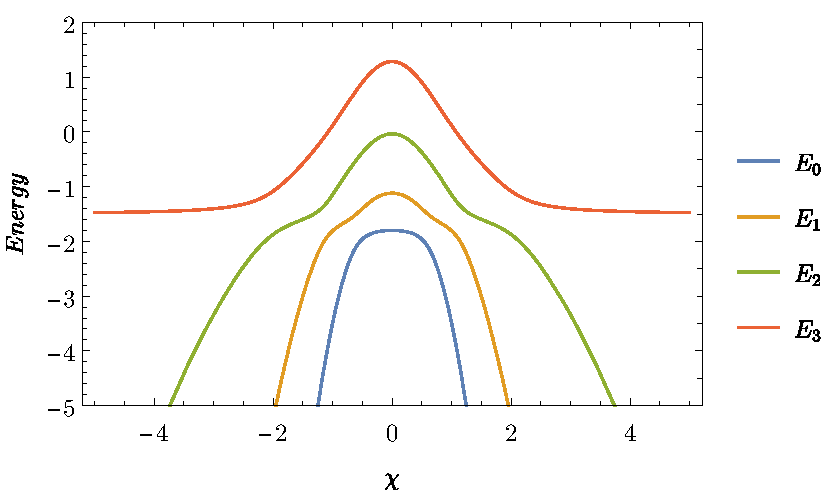
\includegraphics{../img/N=3_energiesl.pdf}
    \caption{Energy for the case $N=3$, section $\lambda=1$}
    \label{fig:N=3_energiesl}
\end{figure}
\begin{figure}[H]
    \centering
    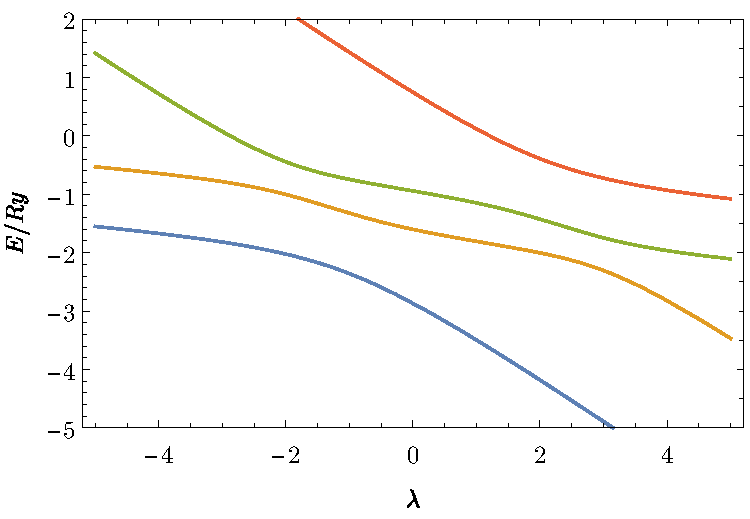
\includegraphics{../img/N=3_energiesc.pdf}
    \caption{Energy for the case $N=3$, section $\chi=1$}
    \label{fig:N=3_energiesc}
\end{figure}

From the Equations \ref{eq:N=3_en0}, \ref{eq:N=3_en1} can be seen that there might exist degeneracy between every two neighboring energy levels\footnote{If the functions $D,E,F,G$ were real numbers, degeneracies would exist between every two neighboring energy levels. Because they are complex, the solution $E_i=E_j$ might not exist. Even though we will see that it's probably not that case and degeneracy exist between every two neighboring energy levels.}. Specifically, for $E_0=E_1$ for $D=E$, which for real values $\lambda,\;\chi$ has two solutions
$$(\lambda_d,\pm \chi_d)=\left(-\frac{1}{2};\sqrt{\frac{3}{5}}\right).$$
Point-like characteristics correspond to Theorem \ref{thm:n-2}, which states that Hamiltonian driven by two real parameters can be degenerated only on 0-dimensional manifolds. 

If the energy spectrum is degenerate and the metric tensor diverges, see individual elements in Fig. \ref{fig:N=3_g}, its determinant also diverges, as shown in Fig. \ref{fig:N=3_gDivenrgence}, along with Christoffel symbols in Fig. \ref{fig:N=3_G}. Note that the metric tensor determinant is positive definite, thus the manifold is Riemannian. Further on, it reflects the symmetry $\chi\leftrightarrow-\chi$, except for elements $g_{12}$, $\Gamma_{121}$, $\Gamma_{211}$, and $\Gamma_{222}$, which switch their sign.
\begin{figure}[H]
    \centering
    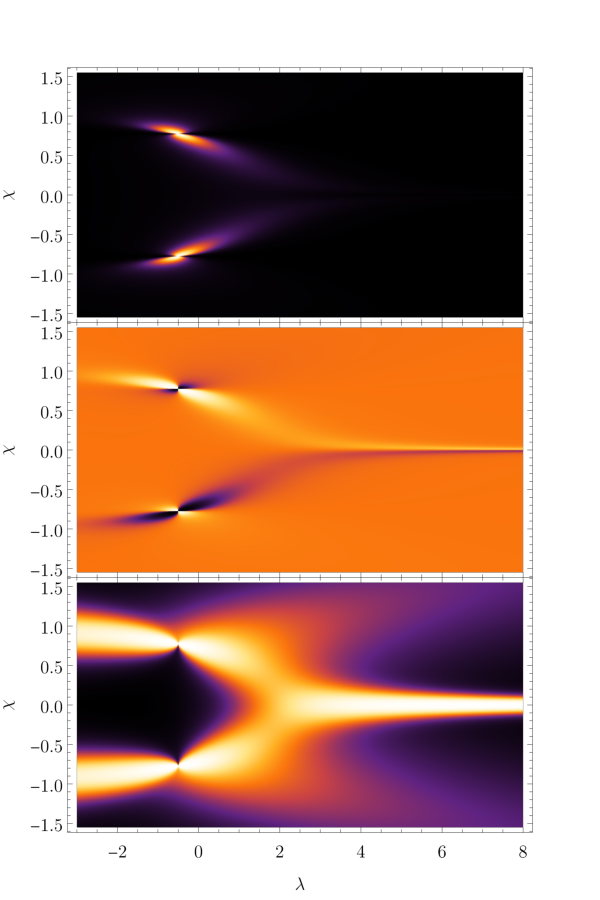
\includegraphics[scale=1.3]{../img/N=3_gComponents.pdf}
    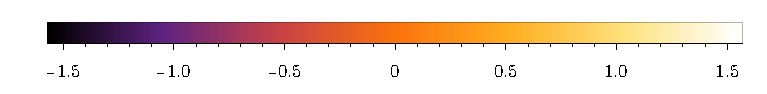
\includegraphics[scale=1.3]{../img/N=3_barA.pdf}
    \caption{Arctangent of the metric tensor elements for the case $N=3$ in the parametric space. From the top: $\arctan(g_{11})$, $\arctan(g_{12})=\arctan(g_{21})$, $\arctan(g_{22})$}
    \label{fig:N=3_g}
\end{figure}


\begin{figure}[H]
    \centering
    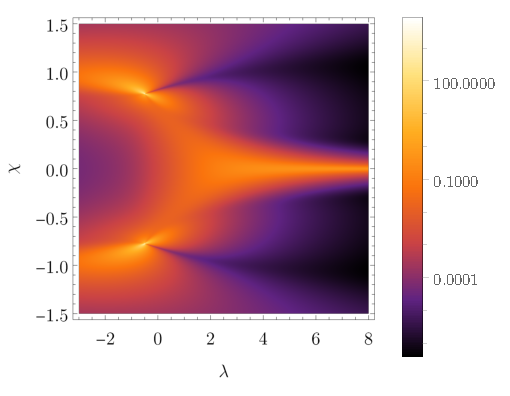
\includegraphics[scale=1.3]{../img/N=3_gDivergence.pdf}
    \caption{Ground state metric tensor determinant in a parametric space for $N=3$.}
    \label{fig:N=3_gDivenrgence}    
\end{figure}

\vspace{-40pt}
\begin{figure}[H]
    \centering
    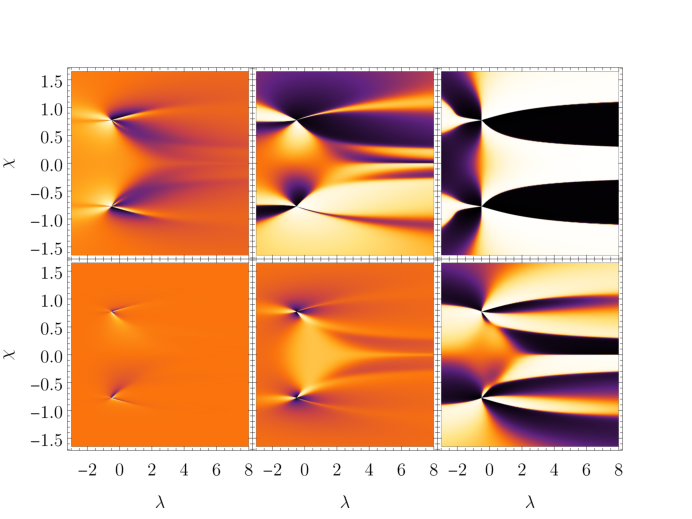
\includegraphics[scale=1.3]{../img/N=3_gammas.pdf}    
    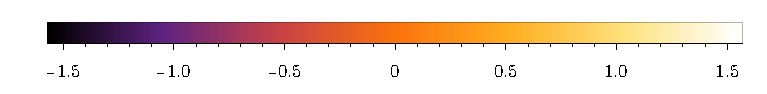
\includegraphics[scale=1.3]{../img/N=3_barA.pdf}
    \caption{Arctangent of the ground state Christoffel symbols for the case $N=3$. First row from left: $\arctan(\Gamma_{111})$, $\arctan(\Gamma_{121})$, $\arctan(\Gamma_{122})$. Second row from left: $\arctan(\Gamma_{211})$, $\arctan(\Gamma_{221})$, $\arctan(\Gamma_{222})$.}
    \label{fig:N=3_G}
\end{figure}

Due to the metric tensor degeneracy, the space is not geodesically maximal. To see that the singularity is not the only \emph{coordinate one}\footnote{Coordinate singularity is present only in some coordinates. This is different from so-called \emph{physical singularity}, which is present in every choice of the coordinate system.}, the Ricci scalar can be calculated, see Fig. \ref{fig:N=3_Ricci}. Divergent Ricci scalar implies the existence of a \emph{physical singularity}. This can be seen from the sections in $\chi$-direction drawn in Fig. \ref{fig:N=3_Ricci_section}, which at coordinate $(\lambda_d;\chi_d)$ diverges. This implies the singularity is \emph{physical}. 

\red{Not sure if true: Note that the energy spectrum degeneracy itself does not imply the metric tensor singularity. For example if the singularity would be only in one point, one might choose inverse radial coordinates. This would move the degeneracy to infinity, which can be removed as a boundary.}



\begin{figure}[H]
    \centering
    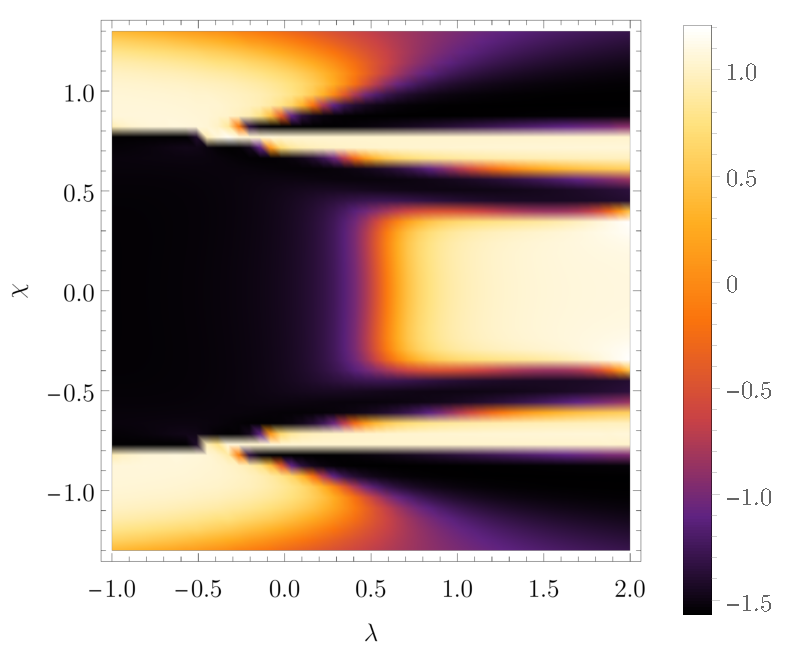
\includegraphics{../img/N=3_Ricci.pdf}
    \caption{Arctangent of Ricci curvature for the case $N=3$. \textcolor{red}{increase the resolution}}
    \label{fig:N=3_Ricci}
\end{figure}

% Coordinates of minima on lines with constant $\lambda$ in Ricci scalar can be seen in Fig. \ref{fig:N=3_RicMinimas} and will be important later on, because geodesics will be strongly repelled by parts of this line.
\begin{figure}[H]
    \centering
    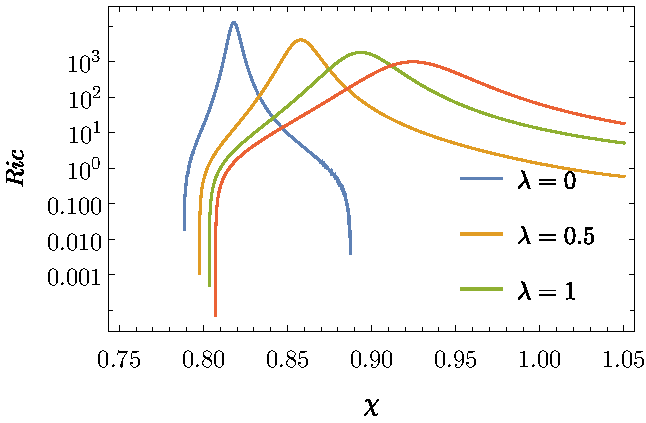
\includegraphics[scale=0.9]{../img/N=3_Ricci_section.pdf}
    \caption{Ricci's curvature sections for three different $\lambda$.}
    \label{fig:N=3_Ricci_section}
\end{figure}
% \begin{figure}[H]
%     \centering
%     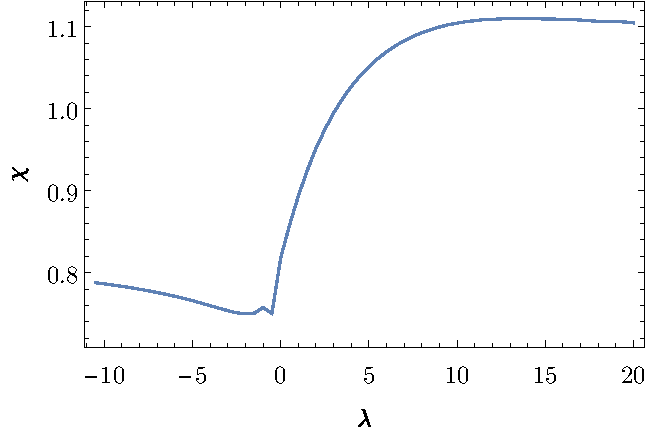
\includegraphics[scale=0.9]{../img/N=3_RicMinimas.pdf}
%     \caption{Minimas in Ricci curvature on the background of metric tensor determinant. Case $N=3$.}
%     \label{fig:N=3_RicMinimas}    
% \end{figure}

Some of the system characteristics can be seen from geodesics. \emph{Initial valued Geodesics} are solutions to
$$(\lambda(T_i);\chi(T_i))\eqqcolon (\lambda_i;\chi_i)\in \R^2$$
$$\left(\der{\lambda(t)}{t};\der{\chi(t)}{t}\right)\Bigg|_{T_i} \eqqcolon (\lambda'_i;\chi'_i) \in \R^2_+,$$
where $T_i$ is \emph{initial time}, typically $0$. 

We might also choose \emph{boundary valued geodesics} with fixed initial $(\lambda(0);\chi(0))$ and final position $(\lambda(T_f);\chi(T_f))$. Because the shape of geodesics in parametric space does not depend on the initial derivative, it does not depend on the speed of driving in the parametric space. Initial valued geodesics are therefore more advantageous to calculate, because they have only two free parameters - the initial coordinate $(\lambda;\chi)$. Another reason is purely numeric, because the boundary valued geodesics are calculated by numerous evolutions of initial valued geodesics with response initial parameter tweaking. This makes the calculations slower (in our case they were $10$ to $100$ times slower).

Results for the geodesics starting at $(\lambda_i;\chi_i)=(0;0)$, $
(\lambda',\chi')=(\cos\theta;\sin\theta)$ can be seen in Fig. \ref{fig:N=3_geodesics}. Other values $\theta$ result in a close approach of the geodesics to the singularity, making the calculations numerically unstable. The fact that geodesics lean towards singularities is well known from the theory of General Relativity (GR). The main difference here is that our "test particle" seems to be partially repulsed by the singularity. The analogy with GR would therefore fail because of the nonexistence of negative mass and gravitational dipoles. The better analogy would be electromagnetism, which has a downside in the fact that the geometrical formalism is not used so much in this theory. Comparison of those two intuitive examples can be seen in Fig. \ref{fig:geodesicsinGR}. The geodesic behavior is not caused only by the singularity but also by a large Ricci curvature leaning to the right from it. This means that the distance across this \emph{\blueee{unreachable gap}}, marked by \blueee{blue line} in Fig. \ref{fig:N=3_geodesics}, is also large. This leads to the strong tendency of geodesics to go around the singularity rather than crossing it. The presence of singularities means that our ground state manifold is geodesically incomplete and according to Theorem \ref{thm:hopf-Rinow_modified} there exist some geodesically unreachable coordinates. From this goes the term \emph{\blueee{unreachable gap}}.



\begin{figure}[H]
    \centering
    % 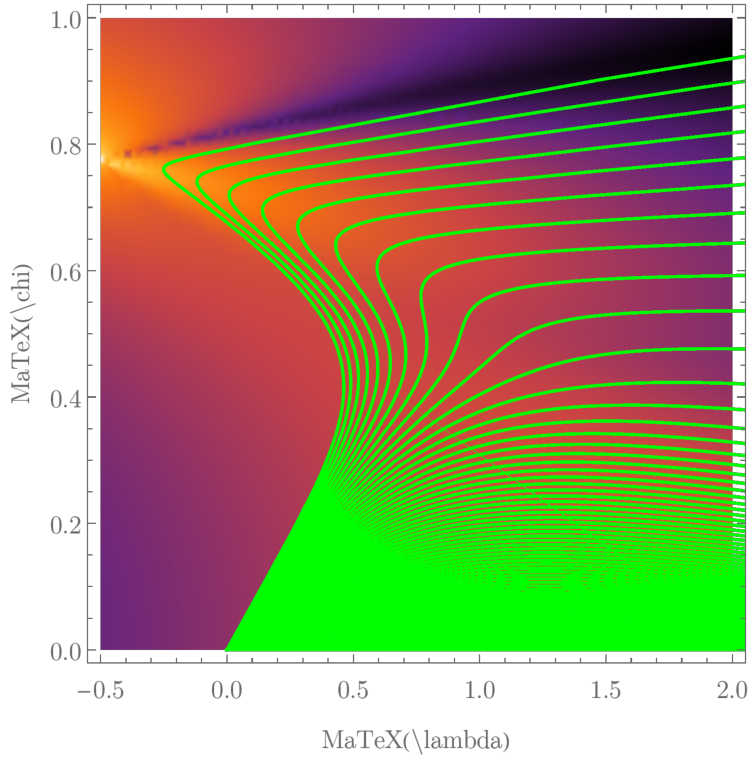
\includegraphics{../img/N=3_geodesics.pdf}
    \begin{tikzpicture}
        \node[anchor=south west,inner sep=0] at (0,0) {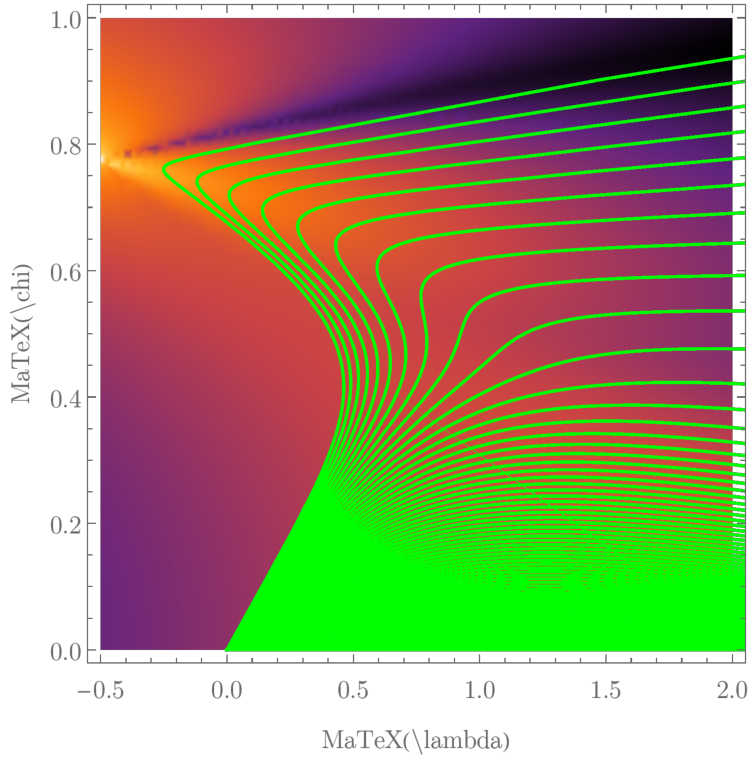
\includegraphics{../img/N=3_geodesics.pdf}};
        \draw[blueee,ultra thick] (4.5,9.56) -- (10.67,10.5);
        \draw[blueee,ultra thick] (4.5,2.71) -- (10.67,1.8);
    \end{tikzpicture}
    \caption{\green{Geodesics} for the case $N=3$ starting from $(\lambda_i;\chi_i)=(0;0)$ with $(\lambda'_i;\chi'_i)=(\cos\theta;\sin\theta)$, parametrized by angle $\theta\in [-0.63;0.63]$, $\theta\in [\pi-0.225;\pi+0.225]$, with step $\Delta\theta=0.01$. \blueee{Blue} line marks the high Ricci curvature gap.}
    \label{fig:N=3_geodesics}    
\end{figure}



\begin{figure}[H]
    \centering
    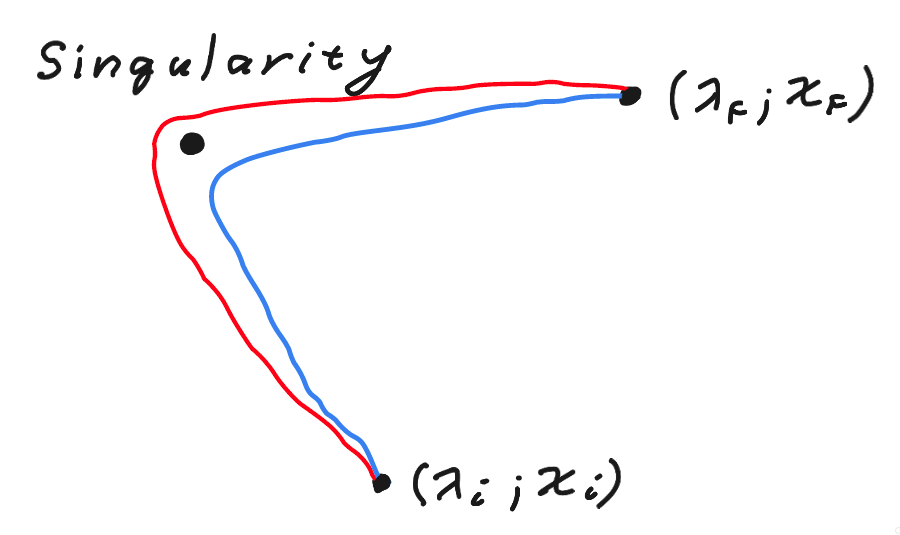
\includegraphics[width=0.6\textwidth]{../img/geodesicsinGR.png}
    \caption{Comparing geodesics with \blue{repulsing (blue)} and \red{attracting (red)} metric tensor divergence in the spherically symmetrical space. }
    \label{fig:geodesicsinGR}
\end{figure}

% \begin{figure}[h]
%     \centering
%     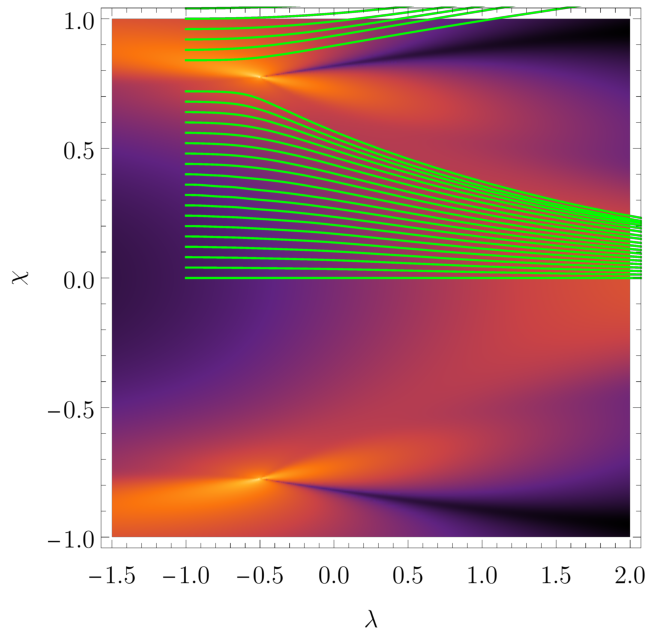
\includegraphics{../img/N=3_geodesics_lambdaIn=-1.pdf}
%     \caption{Geodesics starting from $(\lambda_i;\chi_i)=(-1;\chi_i)$, $(\lambda',\chi')=(1;0)$, for $\chi_i\in(0;1)$ with step $0.05$. Numerically unstable geodesics were skipped. Case $N=3$.}
%     \label{fig:N=3_geodesics_lambdaIn=-1}    
% \end{figure}





\subsection{Case $N=5$}

Another special case is $N=5$. From analysis of the energy levels, we see that there are more degeneracies, see Fig. \ref{fig:singularitiesBetweenEnergiesN=5}. One can see that only $E_0=E_1$ the degeneracy lies on the separatrix and all others are distributed around. The $\chi\leftrightarrow-\chi$ symmetry holds for all of them. 

Another fact, which is good to realize, is how the space itself looks like. This is best seen from the metric tensor determinant, fig. \ref{fig:N=5_det3D}.



\begin{figure}[H]
    \centering
    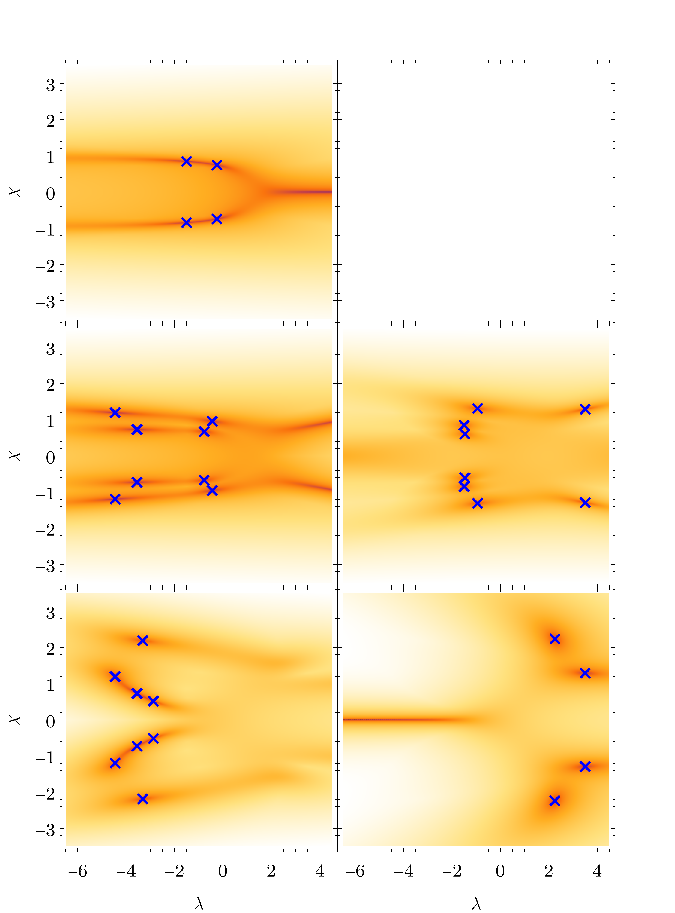
\includegraphics[scale=1.3]{../img/singularitiesBetweenEnergiesN=5.pdf}
    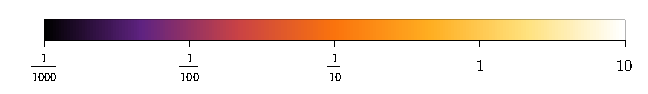
\includegraphics[scale=1.3]{../img/N=5_bar6.pdf}
    \caption{Energy differences between neighboring energy levels for $N=5$. First row: $E_1-E_0$, second row: $E_2-E_1$, $E_3-E_2$, third row: $E_4-E_3$, $E_5-E_4$. Spectra degeneracies are marked with \blue{blue} cross.}
    \label{fig:singularitiesBetweenEnergiesN=5}    
\end{figure}

\begin{figure}[H]
    \centering
    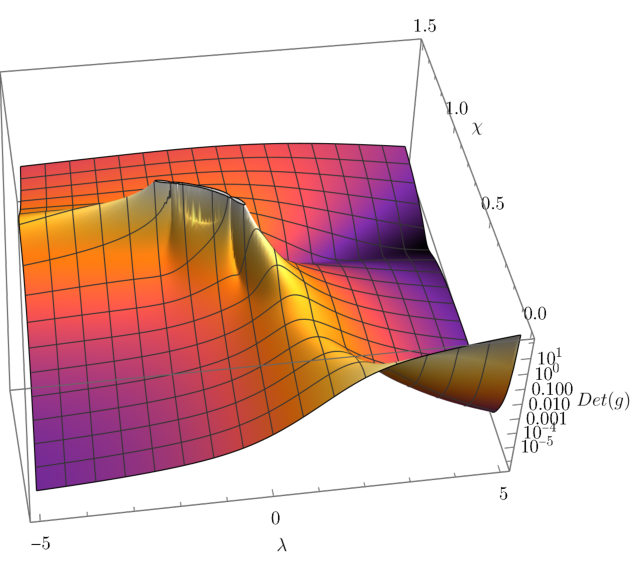
\includegraphics[scale=1.3]{../img/N=5_det3D.pdf}
    \caption{Metric tensor determinant for the case $N=5$.}
    \label{fig:N=5_det3D}    
\end{figure}



Geodesics for the case $N=5$ starting from the point $(0;0)$ have the characteristics already seen in the case $N=3$. However, when starting at $(\lambda;\chi)=(1;0)$, the behavior around the singularity is not the only interesting thing happening. As can be seen in Fig. \ref{fig:geod10}, the geodesics tend to deflect themselves from the area with high curvature around the axis $\chi=0$, which happens even for other initial conditions, just that for $(0;0)$ it is not so apparent. Small irregularity can be seen in Fig. \ref{fig:N=3_geodesics} around $(0.5;0.1)$. This implies that the geodesic equation might have at least two solutions as candidates for the globally shortest path between two points.\footnote{One might recall the effect of gravitational lensing here. In the presence of any mass in the spacetime, there exists more possible light paths (solutions to the geodesic equation) between two points, differing by the initial condition.} 



\begin{figure}[H]
    \centering
    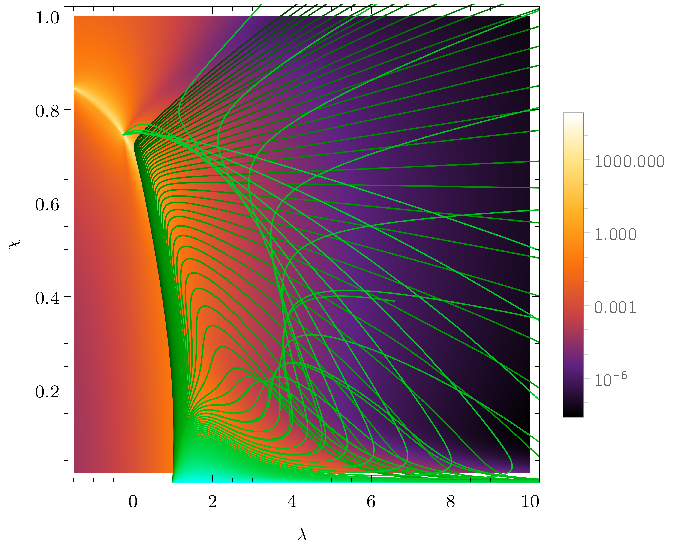
\includegraphics[scale=1.3]{../img/N=5_geods00.pdf}
    \caption{Geodesics for the case $N=5$, starting from the point $(1;0)$. \emph{The numerics around the singularity breaks down, but the solution is close to the drawn one, i.e. they will pass close to the singularity and continue to the left.}}
    \label{fig:geod10}    
\end{figure}

% \begin{figure}[H]
%     \centering
%     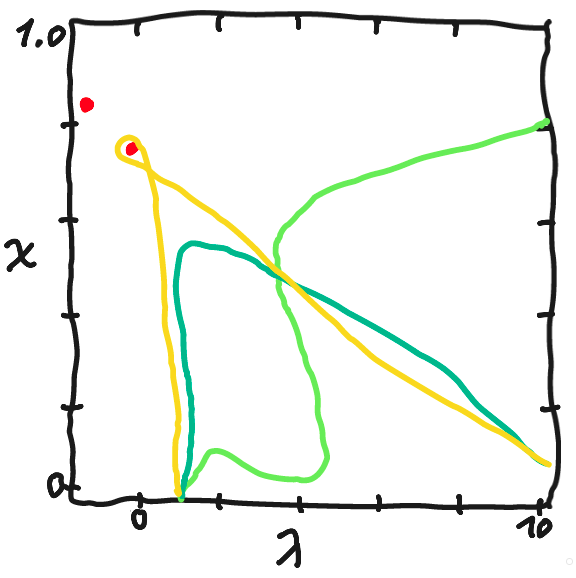
\includegraphics[scale=0.35]{../img/geodesicSolutionsDrawing.png}
%     \caption{Three possible solutions between points $(1;0)$ and $(4;0.5)$. The length of the yellow one is surely longer than other two, but the difference between green vs. blue solution is not clear on the first sight.}
%     \label{fig:geodesicsBetweenPoints}    
% \end{figure}






\subsection{Limit \texorpdfstring{$N\rightarrow \infty$}{N->infty}}
The limit $N\rightarrow \infty$ can be applied to the Hamiltonian in Eq. \ref{eq:firstOrderTransitionHamiltonian} using Holstein-Primakoff mapping\red{cite something} for bosonic operators
\begin{equation}
    \mathcal{H}\coloneqq\lim_{j\rightarrow\infty}\frac{\HH}{2j},
\end{equation}
resulting in classical Hamiltonian
\begin{equation}
    \begin{split}
        \mathcal{H}(x,p)=&-\frac{1}{2}+\frac{1-\lambda}{2}x^2+\frac{\lambda-\chi^2}{4}x^4-\frac{\chi x^3}{2}\sqrt{2-x^2-p^2}-\frac{\chi^2}{4}p^4\\
        &+\frac{p^2}{4}\left[2+(\lambda-2\chi^2)x^2-2\chi x\sqrt{2-x^2-p^2}\right].
    \end{split}
    \label{eq:HamiltonianClassicalLimit}
\end{equation}


Finding minimas in its derivatives, we get the \emph{separatrix}
\begin{equation}
    \chi^2=\frac{\lambda-1}{\lambda-2},
    \label{eq:separatrix}
\end{equation}
which represents the phase transition in the limit $N\rightarrow \infty$. In our case, the transition is of first order everywhere, except in $(\lambda;\chi)=(1;0)$, where it has order two. The separatrix is shown in Fig. \ref{fig:transitionCompare} compared to minimum between the ground state and the first excited state $E_1-E_0$ for $N=3$ case. With increasing $N$, it converges to the separatrix line.

\begin{figure}[H]
    \centering
    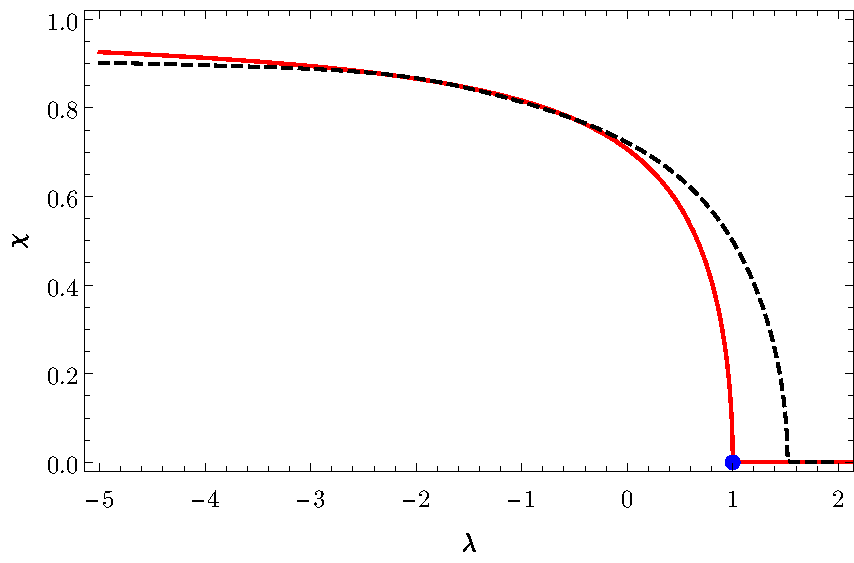
\includegraphics{../img/infiniteN_transitionCompare.pdf}
    \caption{\red{First order phase transition, the Separatrix} (red), \blue{second order transition} (blue point) compared to \emph{minimum between the ground state and first excited state in N=3 case} (black, dashed).}
    \label{fig:transitionCompare}    
\end{figure}












\section{General behavior}
For higher dimensions we see the same characteristic behaviour in the energy spectrum sections, see the example in Fig. \ref{fig:N=10_energiesl}, \ref{fig:N=10_energies2} for the $N=10$ case. Between \textcolor{red}{all} energy levels there is at least one avoided crossing \textcolor{red}{and between zeroth and the first there are $N-2$ crossings for $N$ odd and $N-3$ for $N$ even, which I have no idea how to prove, but it looks like it might be true.}


\begin{figure}[H]
    \centering
    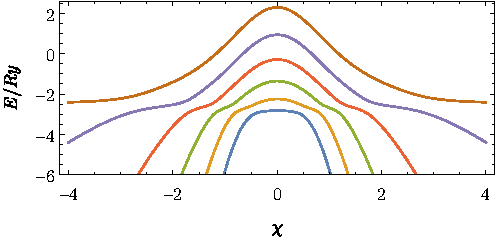
\includegraphics{../img/N=10_energiesl.pdf}
    \caption{Energy spectrum as function of $\chi$, for $\lambda=1$ and $N=10$.}
    \label{fig:N=10_energiesl}    
\end{figure}
\begin{figure}[H]
    \centering
    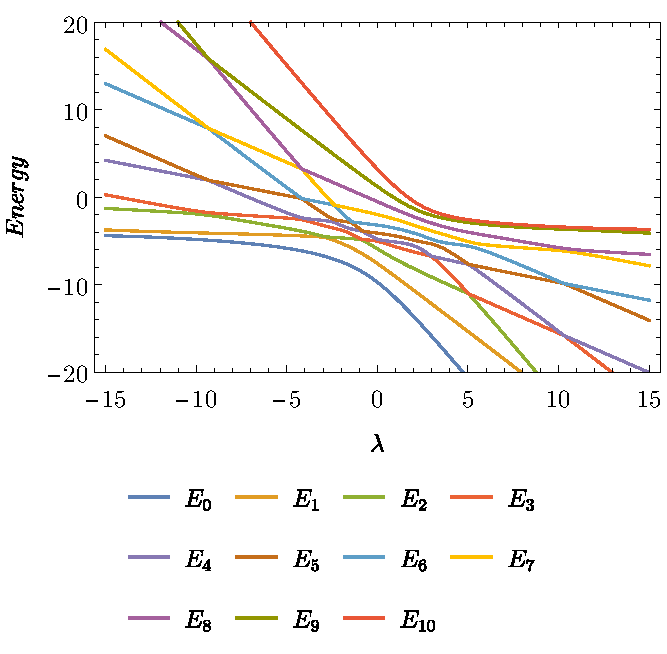
\includegraphics{../img/N=10_energies2.pdf}
    \caption{Energy spectrum as a function of $\lambda$, for $\chi=1$ and $N=10$.}
    \label{fig:N=10_energies2}    
\end{figure}

Special attention was given to the spectrum degeneracies between the zeroth and the first energy level, because those influence the metric tensor and geodesics. Their exact calculation is numerically costly, and only the first few cases, namely, $N\in\{3,4,5,6,7\}$, were calculated, see Tab. \ref{tab:singularities}. 
\begin{table}[H]
    \centering
    \begin{tabular}{c||c|c|c}
     N&$(\lambda_l;\pm\chi_l)$&$(\lambda_2;\pm\chi_2)$&$(\lambda_r;\pm\chi_r)$        \\ \hline\hline
     3&$(-\frac{1}{2};\sqrt{\frac{3}{5}}) $&                                       &                                         \\
     4&$(-3          ;\sqrt{\frac{4}{5}}) $&                                       & $(-\frac{1}{3};\sqrt{\frac{4}{7}})$     \\
     5&$(-\frac{3}{2};\sqrt{\frac{5}{7}}) $&                                       & $(-\frac{1}{4};\sqrt{\frac{5}{9}})$     \\
     6&$(-5          ;\sqrt{\frac{6}{7}}) $&$(-1          ;\sqrt{\frac{2}{3}}) $   & $(-\frac{1}{5};\sqrt{\frac{6}{11}})$     \\
     7&$(-\frac{5}{2};\sqrt{\frac{7}{9}}) $&$(-\frac{3}{4};\sqrt{\frac{7}{11}}) $  & $(-\frac{1}{6};\sqrt{\frac{7}{13}})$ 
    \end{tabular}
    \caption{Singularities between the zeroth and first energy levels for dimensions 3--7. Subscript $l(r)$ means the most \emph{left(right)-wise} positioned coordinates in the $(\lambda,\chi)$-plot.}
    \label{tab:singularities}
    \end{table} 

From the singularity behavior in low dimensions, one might see the pattern
 for $(\lambda_l,\chi_l)$ and $(\lambda_r,\chi_r)$, i.e., those with minimal, resp maximal $\lambda$ coordinate is
\begin{equation}
    (\lambda_l ;\pm\chi_l)= \begin{cases}
        \left(1-\frac{N}{2};\sqrt{\frac{N}{N+2}}\right) & , N\geq 3,N\text{ is odd}\\
        \left(1-N;\sqrt{\frac{N}{N+1}}\right) & , N\geq 3,N\text{ is even}
    \end{cases}
    \label{eq:singularityCoordinateFormulaLeft}
\end{equation}
\begin{equation}
    (\lambda_r ;\pm\chi_r)= 
        \left(\frac{1}{1-N};\sqrt{\frac{N}{2N-1}}\right)\quad , N\geq 3.
        \label{eq:singularityCoordinateFormulaRight}
\end{equation}
Those were numerically proven to be singularities for cases up to $N=1000$. 

Dimensions 3 to 10 are shown in Fig. \ref{fig:singularities3to10}.
In addition, the degeneracies between the zeroth and the first energy levels belong to the separatrix described by Eq. \ref{eq:separatrix}. Due to this, the position of the singularities is constrained to the \emph{second order phase transition line} between points $(\lambda_l,\pm\chi_l)$ and $(\lambda_r,\pm\chi_r)$.



In the limit $N\rightarrow\infty$ they converge to
\begin{align*}
    \lim_{N\rightarrow \infty}(\lambda_l ;\pm\chi_l)&= \left(-\infty,1\right)\\
    \lim_{N\rightarrow \infty}(\lambda_r ;\pm\chi_r)&= \left(0,\frac{1}{\sqrt{2}}\right).
\end{align*}

This means that the whole separatrix is not divergent in the limit $N\rightarrow \infty$. For that the $\chi_r\rightarrow 0$ limit would be needed. Because for $N\rightarrow\infty$ there is an infinite number of singularities and because the whole separatrix is divergent, they need to be dense. \red{this is contradiction, so either the whole separatrix is not divergent, or there appear some points right from $\lambda_r$.}



\begin{figure}[H]
    \centering
    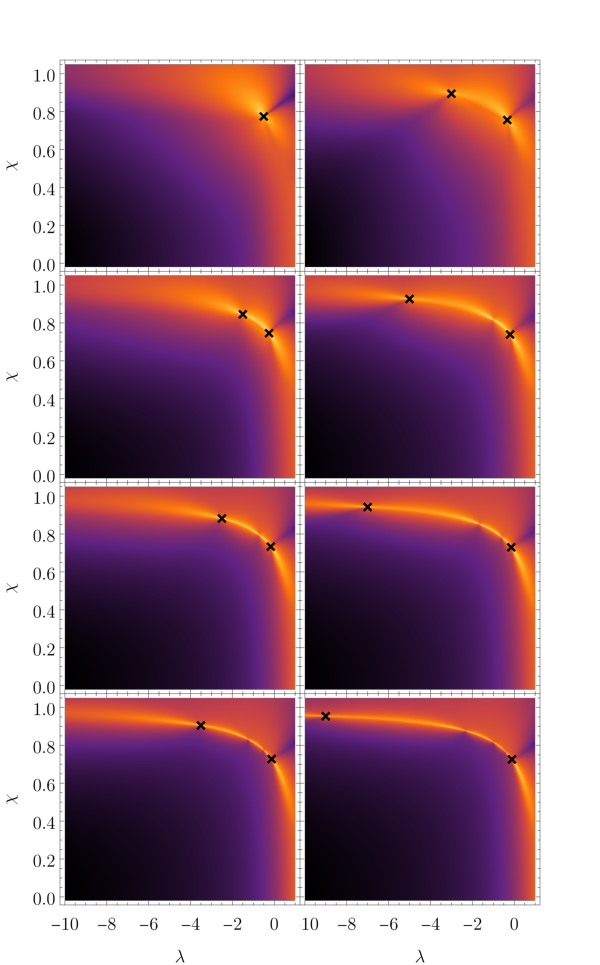
\includegraphics[scale=1.3]{../img/singularitiesPlots.pdf}
    \caption{Spectrum degeneracies between $E_0$ and $E_1$. Hamiltonian dimensions are 1,3,5,7 in the first column and 2,4,6,8 in the second column. Black crosses mark most left-wise and right-wise singularity and the background corresponds to the metric tensor determinant. Other singularities are also well visible in the determinant.}
    \label{fig:singularities3to10}    
\end{figure}









% \section{Higher state manifolds}



% \begin{figure}[H]
%     \centering
%     \includegraphics[scale=1.2]{../img/N=5_metricDeterminants.pdf}
%     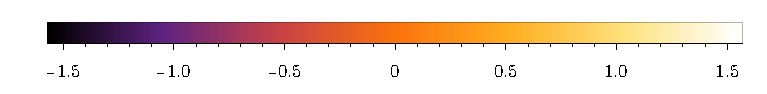
\includegraphics[scale=1.2]{../img/N=3_barA.pdf}
%     \caption{Arctangens of the metric tensor for higher state manifolds. By  rows: $M_0$, $M_1$; $M_2$, $M_3$; $M_4$, $M_5$.}
%     \label{fig:higherStateManifolds}    
% \end{figure}


% \begin{figure}[H]
%     \centering
%     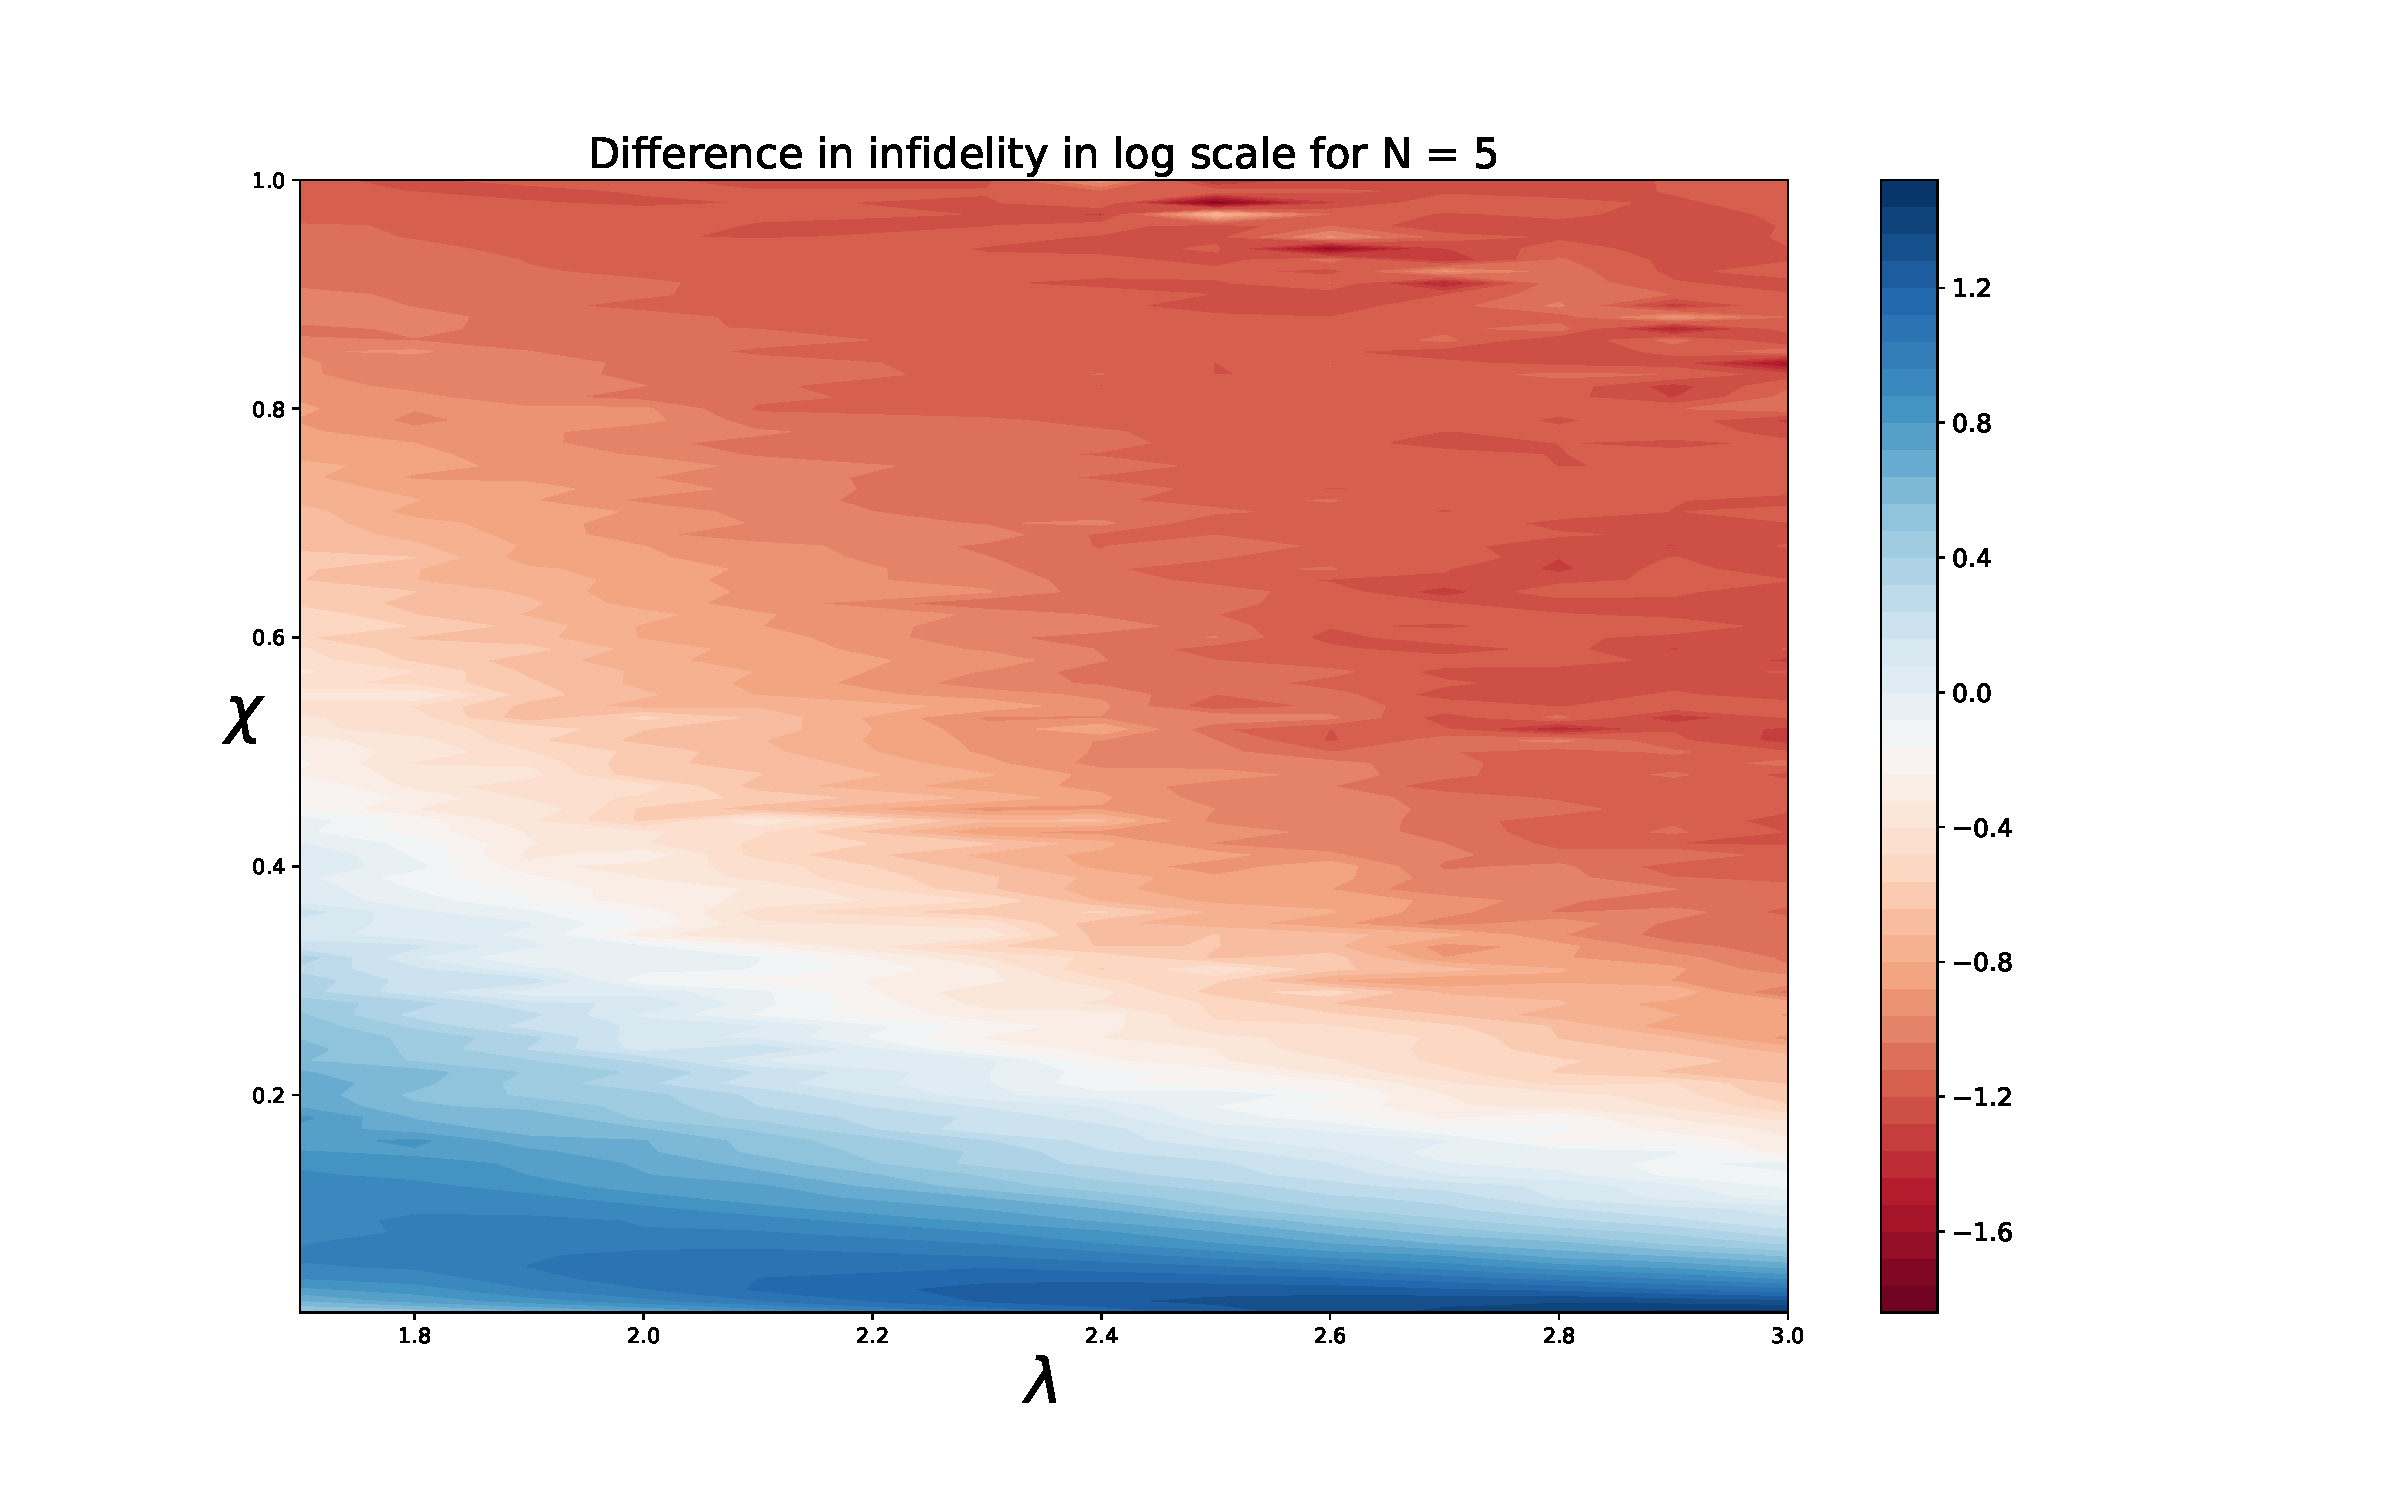
\includegraphics[width=1\textwidth]{../img/fidelity_lineVSgeodesic.pdf}
%     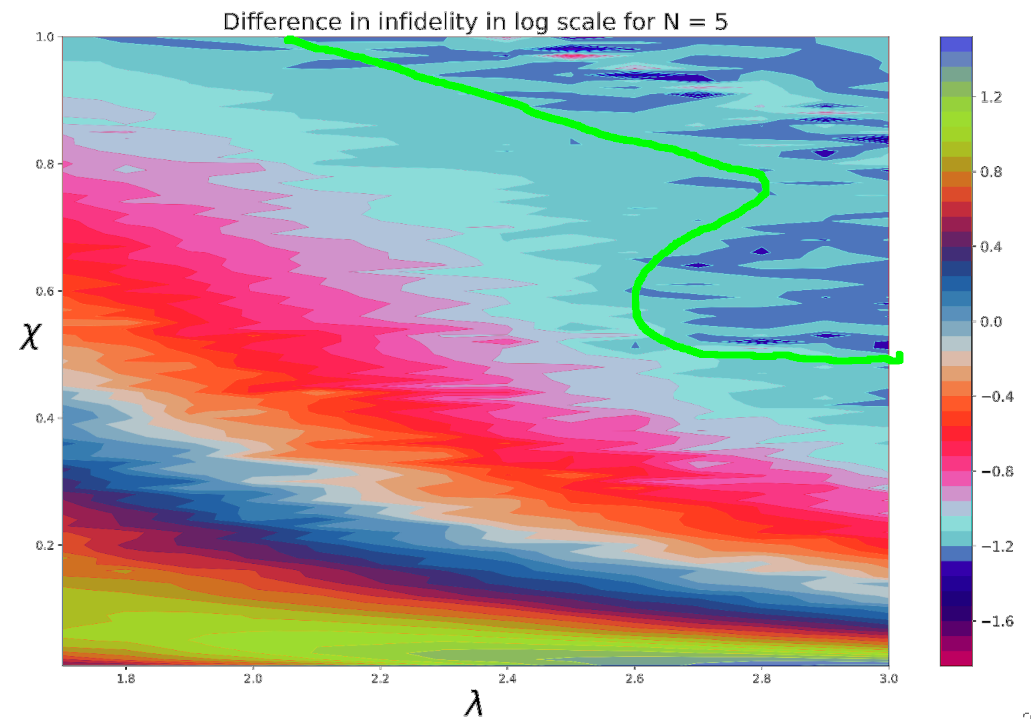
\includegraphics[width=0.8\textwidth]{../img/fidelity_geodesicVSline_fuckedupcolors.png}
%     \caption{\textcolor{gray}{Infidelity difference between line and geodesic, above picture is original from Felipe, bottom one is edited in GIMP to see the difference more clearly.}}
%     \label{fig:higherStateManifolds}    
% \end{figure}
